\section{Plano de fundaciones}
La Figura~\ref{fig:planta_general} presenta la planta general de fundaciones del sector, con la disposición en ejes de los 21 muros y las 9 columnas, el acotado de las dimensiones $B \times L$ obtenidas para cada elemento y los esfuerzos de diseño que controlaron su dimensionamiento. La numeración de ejes corresponde a la empleada en el modelo estructural, consistente con las Tablas~\ref{tab:excentricos} y~\ref{tab:dimpres}.

\begin{figure}[H]
\centering
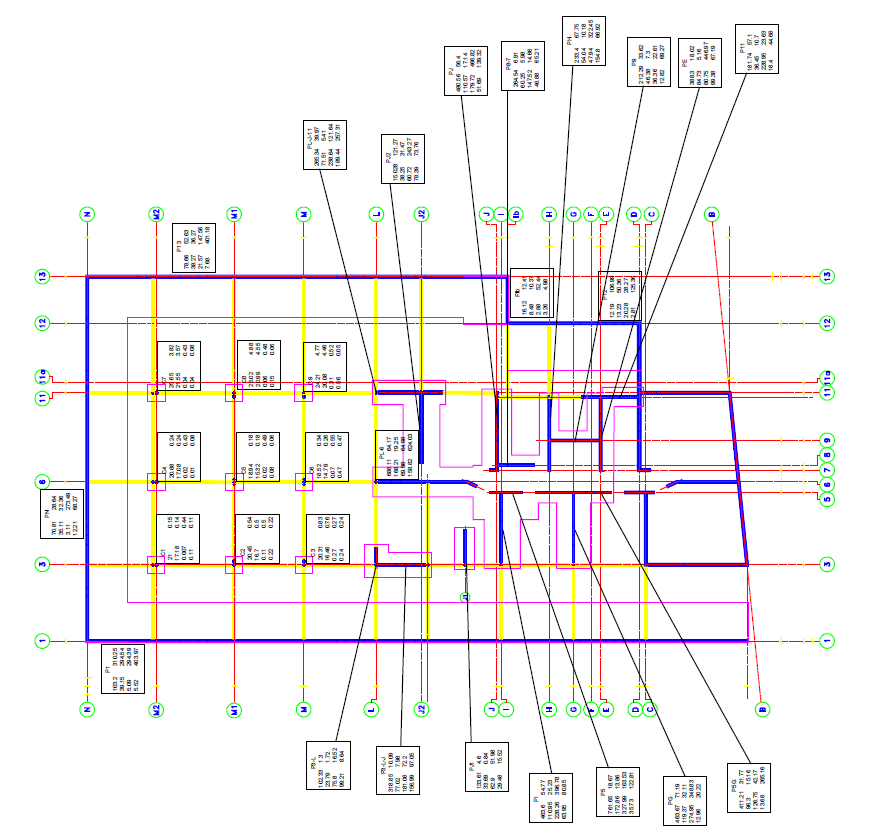
\includegraphics[width=\textwidth]{Secciones/imagenes/general.png}
\caption{Planta general de fundaciones, con acotado de dimensiones y esfuerzos de diseño por elemento.}
\label{fig:planta_general}
\end{figure}

Las Figuras~\ref{fig:corte_perimetral} y~\ref{fig:corte_corrida} presentan los cortes tipo de zapata adoptados. La Figura~\ref{fig:corte_perimetral} corresponde al muro P1, representativo de los muros perimetrales con zapata excéntrica: se observa el muro situado en el borde exterior de la zapata, con la base desarrollándose únicamente hacia el interior en un ancho $B = 2,85$~m y altura $H = 1,20$~m, y la armadura principal $\phi 18 @ 100$~mm dispuesta en ambas direcciones. La Figura~\ref{fig:corte_corrida} corresponde a una zapata corrida centrada, representativa de los muros interiores, con el muro ubicado en el eje de la base.

\begin{figure}[H]
\centering
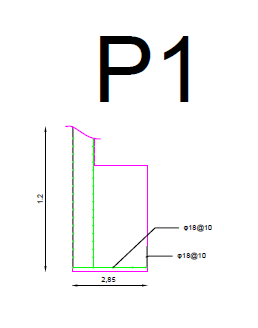
\includegraphics[width=0.45\textwidth]{Secciones/imagenes/perimetral.png}
\caption{Corte tipo de zapata excéntrica, muro perimetral P1.}
\label{fig:corte_perimetral}
\end{figure}

\begin{figure}[H]
\centering
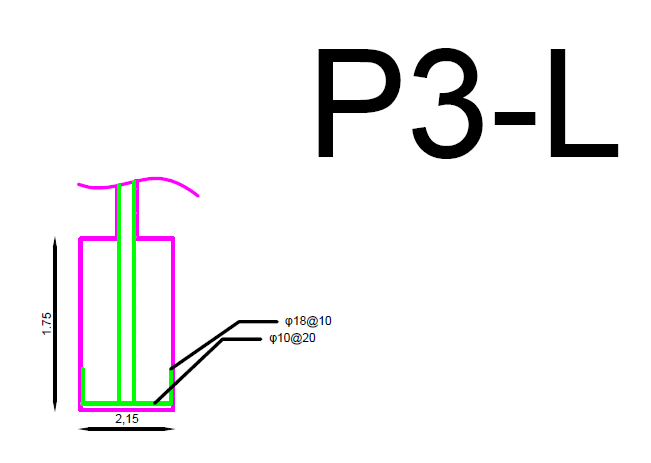
\includegraphics[width=0.45\textwidth]{Secciones/imagenes/corrida.png}
\caption{Corte tipo de zapata corrida centrada, muro interior.}
\label{fig:corte_corrida}
\end{figure}